\chapter{Contexte général}


\chapteropeningtext{Ce chapitre présente le cadre général dans lequel s'inscrit le projet réalisé durant le stage de fin d'études. Il introduit d'abord l'organisme d'accueil ainsi que le contexte organisationnel du stage. Il décrit ensuite la situation existante liée au suivi des camions loués transportant la ferraille depuis le port vers l'usine, puis met en évidence les limites du processus actuel et la problématique à résoudre. Par la suite, ce chapitre présente la solution proposée, ses principaux objectifs, ainsi que la méthodologie de travail adoptée et les grandes phases de planification du projet.}{Contexte industriel -- SOMASTEEL -- Problématique -- Objectifs -- Planification}

\section{Organisme d'accueil et contexte du stage}

Le stage de fin d'études a été réalisé au sein de \textbf{SOMASTEEL}, une entreprise marocaine de référence dans le secteur de la sidérurgie. Fondée en 2007, SOMASTEEL est spécialisée dans le laminage à chaud des aciers et la fabrication de fer rond à béton destiné principalement au secteur du bâtiment. L'entreprise dispose d'un site industriel important à Oulad Azzouz, à Casablanca, ainsi que d'une nouvelle aciérie située à Nouaceur.

SOMASTEEL exerce son activité dans un secteur industriel où la continuité de la production dépend fortement de la disponibilité des matières premières et de l'efficacité des flux logistiques. La ferraille constitue une matière première essentielle dans le processus de production. Elle est notamment importée par voie maritime, puis transportée depuis le port vers le site industriel de l'entreprise à l'aide de camions loués.

Selon les informations internes communiquées dans le cadre du stage, SOMASTEEL est une société à responsabilité limitée opérant dans la sidérurgie, avec un chiffre d'affaires avoisinant 4 milliards de dirhams et un effectif pouvant atteindre environ 900 employés. Ces éléments traduisent l'importance de l'activité industrielle de l'entreprise et la nécessité de disposer de solutions numériques adaptées à ses besoins opérationnels.

Sur le plan organisationnel, le projet a été réalisé dans un contexte de collaboration entre la \textbf{Direction des Systèmes d'Information} et le \textbf{service logistique}. La Direction des Systèmes d'Information joue un rôle transversal en accompagnant les différents services métiers dans la digitalisation de leurs processus. Le service logistique représente, dans ce projet, le service bénéficiaire de la solution, puisqu'il est directement concerné par le suivi des camions transportant la ferraille.

Le stage s'est déroulé sur une période de deux mois. Durant cette période, j'ai été chargé de concevoir et développer une solution digitale permettant de répondre au besoin de suivi des camions loués. Le projet a été réalisé individuellement, sous l'encadrement du manager de la Direction des Systèmes d'Information. Des points de suivi hebdomadaires ont permis de présenter l'avancement du travail, de valider les choix fonctionnels et techniques, et d'obtenir les ressources nécessaires à la réalisation du projet.

\section{Situation existante et problématique}

Dans son activité quotidienne, SOMASTEEL gère deux catégories principales de camions. La première catégorie concerne les camions appartenant à l'entreprise. Ces véhicules sont utilisés principalement pour assurer la livraison des produits finis, notamment les barres de fer à béton. Étant donné qu'ils appartiennent à l'entreprise, ils peuvent être équipés d'un système GPS permettant de suivre leurs déplacements et d'obtenir des informations précises sur leurs trajets.

La deuxième catégorie concerne les camions loués. Ces véhicules sont utilisés pour transporter la ferraille importée depuis le port vers le site industriel de SOMASTEEL. Contrairement aux camions appartenant à l'entreprise, les camions loués ne peuvent pas être équipés d'un dispositif GPS, car SOMASTEEL ne dispose pas de l'autorisation nécessaire pour installer ce type d'équipement sur des véhicules externes.

\begin{figure}[H]
    \centering
    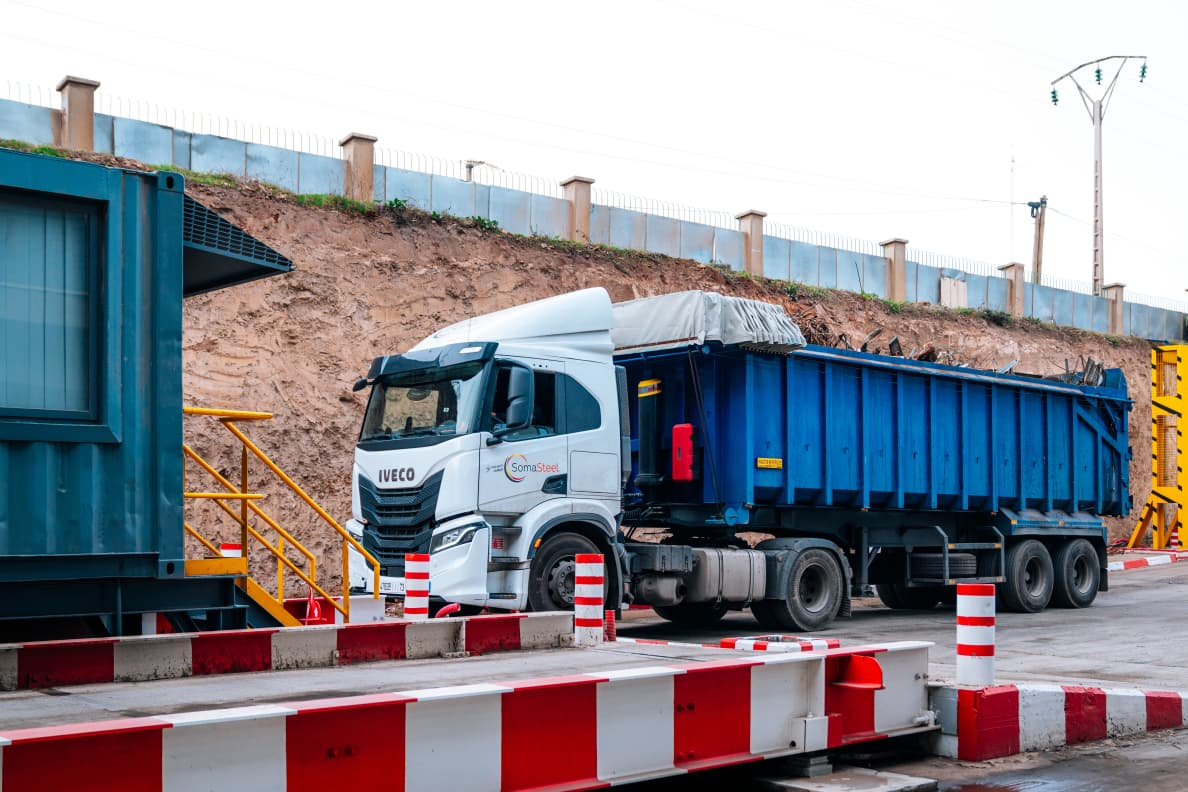
\includegraphics[width=\textwidth,keepaspectratio]
    {figures/screenshots/camions-loues-reels.png}

    \caption{Camions loués utilisés pour le transport de la ferraille}

    \label{fig:camions-loues-reels}
\end{figure}

Avant la mise en place de la solution proposée, le suivi de ces camions loués reposait principalement sur des communications téléphoniques. Ce mode de suivi permettait d'obtenir certaines informations, mais il présentait plusieurs limites. Les informations n'étaient pas centralisées dans un système unique, leur fiabilité dépendait des échanges humains, et il était difficile d'obtenir une vision claire et instantanée de l'état de chaque camion. De plus, le volume des trajets pouvait varier fortement selon l'arrivée des navires transportant la ferraille, ce qui rendait le suivi manuel encore plus complexe.

Le processus d'approvisionnement dépend en effet de l'arrivée des bateaux transportant la ferraille vers le Maroc. Lorsque la marchandise arrive au port, plusieurs camions loués sont mobilisés pour assurer les rotations entre le port et l'usine. À titre d'exemple, durant une période observée entre avril et mai, le nombre de trajets journaliers a pu varier de manière importante, avec 59 trajets le 29 avril, 22 trajets le 30 avril, 40 trajets le 15 mai, 45 trajets le 16 mai, 68 trajets le 17 mai, 83 trajets le 18 mai et 53 trajets le 19 mai. Ces variations montrent l'importance de disposer d'un outil capable d'assurer un suivi fiable, même en période de forte activité.

La problématique principale du projet peut donc être formulée comme suit :

\begin{quote}
Comment concevoir et mettre en place une solution digitale simple, fiable et adaptée aux contraintes de SOMASTEEL, permettant de suivre les camions loués transportant la ferraille depuis le port vers l'usine, sans recourir à un système GPS ?
\end{quote}

Cette problématique implique plusieurs besoins. Le système doit permettre d'identifier chaque camion de manière unique, d'enregistrer les événements importants du trajet, de suivre l'évolution du statut de chaque camion, de centraliser les informations et de fournir au service logistique une visibilité claire sur les expéditions en cours.

\section{Solution proposée et objectifs}

Pour répondre à cette problématique, la solution proposée consiste à développer une application nommée \textbf{SomaScan}. Cette solution repose sur l'identification des camions à l'aide de codes QR associés aux plaques d'immatriculation. Lorsqu'un nouveau camion est ajouté dans le système par l'agent logistique, un code QR unique est généré automatiquement. Ce code peut ensuite être téléchargé et utilisé pour identifier le camion lors des opérations de suivi.

Le principe de fonctionnement de la solution repose sur des points de contrôle. Deux opérateurs interviennent sur le terrain : un opérateur situé au niveau du port et un opérateur situé au niveau de l'usine. Lorsqu'un camion arrive ou quitte un point de contrôle, l'opérateur scanne son code QR à l'aide de l'application mobile. Le système enregistre alors l'événement correspondant et met à jour le statut du camion.

Le workflow initial du système repose sur plusieurs statuts, notamment : \path{STARTED}, \path{ARRIVED_PORT}, \path{LEFT_PORT} et \path{COMPLETED}. Ces statuts permettent de représenter les principales étapes du trajet d'un camion. Toutefois, le fonctionnement peut être adapté selon les besoins opérationnels, par exemple en se concentrant uniquement sur les étapes principales telles que la sortie du port et l'arrivée à l'usine.

La solution est organisée autour de trois acteurs principaux. Les deux premiers sont les opérateurs de terrain, qui utilisent l'application mobile développée avec Flutter pour scanner les codes QR et mettre à jour les statuts des camions. Le troisième acteur est l'agent logistique, qui utilise l'application web d'administration développée avec React afin de gérer les camions, consulter les expéditions et préparer des rapports destinés à la Direction Générale. L'idée initiale du projet a été portée par la Direction Générale, dans le but d'améliorer la visibilité sur le transport de la ferraille et de réduire la dépendance au suivi téléphonique.

Sur le plan technique, la solution est composée de trois parties principales. La première est un backend développé avec Laravel. Il assure la gestion des données, la logique métier, l'authentification basée sur les rôles et l'exposition des API REST. La deuxième partie est une application mobile développée avec Flutter, destinée aux opérateurs du port et de l'usine. La troisième partie est une application web développée avec React, destinée à l'agent logistique pour l'administration et le suivi des opérations.

L'objectif général du projet est de concevoir, développer et déployer une solution digitale permettant à SOMASTEEL de suivre les camions loués transportant la ferraille depuis le port vers l'usine, tout en respectant la contrainte liée à l'impossibilité d'utiliser un système GPS.

Les objectifs spécifiques du projet sont les suivants :

\begin{itemize}
    \item analyser le processus existant de suivi des camions loués ;
    \item identifier les limites du suivi par téléphone ;
    \item proposer une solution alternative basée sur l'identification par code QR ;
    \item concevoir une architecture applicative composée d'un backend, d'une application mobile et d'une application web ;
    \item développer un backend avec Laravel pour gérer les données, les utilisateurs, les rôles et les expéditions ;
    \item développer une application mobile avec Flutter permettant aux opérateurs de scanner les codes QR ;
    \item développer une application web avec React permettant à l'agent logistique de gérer les camions et de suivre les expéditions ;
    \item mettre en place une authentification basée sur les rôles : administrateur, opérateur port et opérateur usine ;
    \item permettre la génération automatique et le téléchargement des codes QR associés aux plaques d'immatriculation ;
    \item centraliser les informations relatives aux trajets et aux statuts des camions ;
    \item faciliter la préparation de rapports destinés à la Direction Générale ;
    \item tester et valider les principales fonctionnalités du système ;
    \item déployer une première version exploitable de la solution ;
    \item proposer un workflow DevOps permettant d'automatiser le déploiement du backend lors de la publication d'une nouvelle version.
\end{itemize}

\section{Méthodologie de travail et planification}

La réalisation du projet a suivi une méthodologie itérative et incrémentale. Cette approche est adaptée aux projets où les besoins peuvent évoluer progressivement en fonction des retours des utilisateurs et des contraintes du terrain. Elle a permis de découper le travail en plusieurs phases, allant de la compréhension du besoin jusqu'à la livraison d'une première version fonctionnelle de la solution.

Le projet a commencé par une phase d'étude du contexte métier. Cette phase a permis de comprendre l'organisation logistique de SOMASTEEL, la différence entre les camions internes et les camions loués, ainsi que les contraintes liées à l'absence de GPS sur les véhicules externes. Elle a également permis d'identifier les acteurs concernés par le système, à savoir les opérateurs du port, les opérateurs de l'usine et l'agent logistique.

La deuxième phase a porté sur l'analyse des besoins et la définition des fonctionnalités principales. Il s'agissait notamment de déterminer les statuts des camions, les actions réalisables par chaque acteur, les données à gérer et les informations nécessaires au suivi des expéditions. Cette phase a servi de base à la conception de l'architecture générale de la solution.

La phase de conception a permis de définir l'organisation technique du système. Le choix s'est porté sur une architecture composée d'un backend Laravel, d'une application mobile Flutter et d'une application web React. Cette séparation permet de centraliser la logique métier au niveau du backend, tout en offrant des interfaces adaptées aux différents utilisateurs du système.

La phase de développement a été réalisée progressivement. Le backend a été mis en place pour gérer les données, l'authentification, les rôles, les camions, les codes QR et les expéditions. L'application mobile a ensuite été développée afin de permettre aux opérateurs de scanner les codes QR et de mettre à jour les statuts des camions. L'application web a été développée pour permettre à l'agent logistique d'administrer les données, de consulter les informations et de préparer les rapports.

Des réunions hebdomadaires avec le manager de la Direction des Systèmes d'Information ont permis de suivre l'avancement du projet, de valider les choix réalisés et de corriger les éventuelles anomalies identifiées. Cette organisation a permis d'améliorer progressivement la solution et de l'adapter aux besoins réels du service logistique.

La planification globale du projet sur les deux mois de stage peut être résumée comme suit :

\begin{table}[H]
\centering
\begin{tabular}{|p{4cm}|p{10cm}|}
\hline
\textbf{Période} & \textbf{Travaux réalisés} \\
\hline
Semaine 1 & Étude du contexte de SOMASTEEL, compréhension du processus logistique et identification du besoin. \\
\hline
Semaine 2 & Analyse de la situation existante, formulation de la problématique et définition des acteurs du système. \\
\hline
Semaine 3 & Conception de l'architecture générale, définition du modèle de données et préparation des principales fonctionnalités. \\
\hline
Semaines 4 et 5 & Développement du backend Laravel, mise en place des API, de l'authentification, des rôles et de la gestion des données. \\
\hline
Semaine 6 & Développement de l'application mobile Flutter pour le scan des codes QR et la mise à jour des statuts. \\
\hline
Semaine 7 & Développement de l'application web React pour l'administration, le suivi des expéditions et la préparation des rapports. \\
\hline
Semaine 8 & Tests, validation, corrections, préparation du déploiement et proposition du workflow DevOps. \\
\hline
\end{tabular}
\caption{Planification globale du projet}
\label{tab:planning-projet}
\end{table}

Cette planification présente les grandes étapes du projet de manière synthétique. Elle met en évidence la progression logique du travail, depuis l'analyse du besoin jusqu'à la réalisation technique et la préparation du déploiement.

\section{Conclusion}

Ce chapitre a présenté le contexte général du projet réalisé au sein de SOMASTEEL. Il a d'abord introduit l'organisme d'accueil, son domaine d'activité et le cadre organisationnel du stage. Il a ensuite décrit la situation existante liée au suivi des camions loués transportant la ferraille depuis le port vers l'usine, en mettant en évidence les limites du suivi par téléphone et l'impossibilité d'utiliser un système GPS sur ces véhicules.

La solution proposée, intitulée \textbf{SomaScan}, repose sur l'identification des camions par codes QR et sur la mise à jour de leurs statuts par des opérateurs situés au port et à l'usine. Elle est composée d'un backend Laravel, d'une application mobile Flutter et d'une application web React. Ce chapitre a également présenté les objectifs du projet, la méthodologie de travail adoptée et la planification globale sur la période du stage.

Le chapitre suivant sera consacré à l'analyse et à la spécification des besoins. Il présentera les acteurs du système, les exigences fonctionnelles et non fonctionnelles, ainsi que les principaux cas d'utilisation de la solution.
